%%%% ijcai25.tex

\typeout{IJCAI--25 Instructions for Authors}

% These are the instructions for authors for IJCAI-25.

\documentclass{article}
\pdfpagewidth=8.5in
\pdfpageheight=11in
\usepackage{xcolor}
% The file ijcai25.sty is a copy from ijcai22.sty
% The file ijcai22.sty is NOT the same as previous years'
\usepackage{ijcai25}

% Use the postscript times font!
\usepackage{times}
\usepackage{soul}
\usepackage{url}
\usepackage[hidelinks]{hyperref}
\usepackage[utf8]{inputenc}
\usepackage[small]{caption}
\usepackage{graphicx}
\usepackage{amsmath}
\usepackage{amsthm}
\usepackage{booktabs}
\usepackage{algorithm}
\usepackage{algorithmic}
\usepackage[switch]{lineno}
\usepackage{comment}
% Comment out this line in the camera-ready submission
%\linenumbers

\urlstyle{same}

% the following package is optional:
%\usepackage{latexsym}

% See https://www.overleaf.com/learn/latex/theorems_and_proofs
% for a nice explanation of how to define new theorems, but keep
% in mind that the amsthm package is already included in this
% template and that you must *not* alter the styling.
\newtheorem{example}{Example}
\newtheorem{theorem}{Theorem}

% Following comment is from ijcai97-submit.tex:
% The preparation of these files was supported by Schlumberger Palo Alto
% Research, AT\&T Bell Laboratories, and Morgan Kaufmann Publishers.
% Shirley Jowell, of Morgan Kaufmann Publishers, and Peter F.
% Patel-Schneider, of AT\&T Bell Laboratories collaborated on their
% preparation.

% These instructions can be modified and used in other conferences as long
% as credit to the authors and supporting agencies is retained, this notice
% is not changed, and further modification or reuse is not restricted.
% Neither Shirley Jowell nor Peter F. Patel-Schneider can be listed as
% contacts for providing assistance without their prior permission.

% To use for other conferences, change references to files and the
% conference appropriate and use other authors, contacts, publishers, and
% organizations.
% Also change the deadline and address for returning papers and the length and
% page charge instructions.
% Put where the files are available in the appropriate places.


% PDF Info Is REQUIRED.

% Please leave this \pdfinfo block untouched both for the submission and
% Camera Ready Copy. Do not include Title and Author information in the pdfinfo section
\pdfinfo{
/TemplateVersion (IJCAI.2025.0)
}

\title{Creative Momentum Transfer: How Timing and Labeling of AI Suggestions Shape Iterative Human Ideation}
\author{
Guangrui Fan$^{1}$\footnote{Corresponding author: Guangrui Fan}
\and
Dandan Liu$^{2}$\and
Lihu Pan$^{1}$\And
Yishan Huang$^{3}$\\
\affiliations
$^{1}$Taiyuan University of Science and Technology\\
$^{2}$Universiti Malaya\\
$^{3}$Beijing Sankuai Network Technology Co., Ltd\\
\emails
fgr@tyust.edu.cn,
s2134717@siswa.um.edu.my,
panlh@tyust.edu.cn,
juewangh13@outlook.com
}
\begin{document}

\maketitle

\begin{abstract}
Human–AI collaboration is increasingly integral to a variety of domains where creative ideation unfolds in iterative cycles, yet most existing studies evaluate AI-generated concepts in a single step. This paper addresses the gap by investigating “Creative Momentum Transfer”—how the timing (early vs. late) and labeling (AI-labeled vs. unlabeled) of AI prompts shape multi-round human ideation. In a between-subjects experiment (\(N = 247\)), participants proposed solutions for plastic pollution over two rounds, with AI suggestions introduced either at the outset or mid-process and labeled explicitly or not. Results reveal that early AI prompts increase overall creativity but induce stronger anchoring, whereas late AI prompts trigger a mid-round pivot that fosters more divergent thinking yet still boosts final outcomes compared to a no-AI control. Labeling amplifies both subjective and objective adoption of AI ideas, although most participants could detect AI sources even when unlabeled. Furthermore, qualitative interviews highlight nuanced perspectives on perceived ownership, authenticity, and the ways in which labeling triggers deeper scrutiny of the AI’s style. By demonstrating that baseline creativity moderates these effects more robustly than trust in AI, this study advances our theoretical understanding of multi-round human–AI synergy while offering design guidelines for next-generation creativity support systems. We discuss how user-centered design can balance rapid convergence (via early AI) with strategic pivot opportunities (via late AI) and weigh transparent labeling against ethical considerations of authorship and user autonomy.
\end{abstract}

\section{Introduction}

Generative AI tools—ranging from large language models to diffusion-based image generators—now produce outputs with near-human or even superior performance in domains such as marketing, product ideation, and technical writing~\cite{epstein2023art,kwon2024designer,reeves2024generative}. By rapidly generating novel ideas, these systems have heightened interest in human–AI collaboration, where people can leverage AI’s breadth of knowledge while preserving human judgment and ethical discretion~\cite{fui2023generative,ma2024human}. Despite the wealth of research on AI-assisted creativity, most existing studies focus on single-step or one-off comparisons—for example, assessing whether AI ideas are more or less creative than solely human-generated ones~\cite{doshi2024generative,burton2024large}.

However, genuine creative endeavors typically unfold iteratively, with ideas introduced, refined, or reoriented across multiple rounds of brainstorming or problem-solving~\cite{tolkamp2023creativity,zamani2022closer}. A single AI-generated suggestion rarely remains static—its influence can build over time as people adapt or diverge from it across multiple ideation phases. Yet we lack a systematic understanding of how the timing (e.g., early vs. late introduction) and labeling (explicitly tagged as “AI-generated” vs. presented without attribution) of these prompts might shape multi-round ideation.

To address this gap, we propose the concept of “Creative Momentum Transfer,” describing how AI-generated inputs can anchor or redirect human thinking over successive rounds of idea development. Our framework builds on cognitive anchoring theory~\cite{tversky1974judgment} and the System I vs. System II model~\cite{kahneman2011thinking}: early AI suggestions may spark fast (System I) assimilation but increase the risk of anchoring, whereas later AI prompts might allow individuals to explore independently first (System II deliberation) and then “pivot” upon encountering external ideas. Furthermore, labeling—explicitly identifying a suggestion as machine-generated—can alter acceptance, trust, and sense of authorship~\cite{brachman2022reliance}.

Although co-creative arts (e.g., music composition, visual arts) exemplify the potential of multi-round human–AI collaboration~\cite{rezwana2023designing}, the impact of timing and labeling also extends to broader contexts such as product design, scientific inquiry, and educational tools, where iterative refinement is common. From a human-centered AI perspective, understanding how and when users incorporate AI prompts is crucial to designing systems that balance rapid ideation with transparency and respect for user autonomy. These considerations address the broader goal of developing AI-driven solutions that are beneficial, adaptable, and ethically responsible. 

In this research, plastic pollution serves as an illustrative domain precisely because tackling it requires sustained, multi-pronged solutions—mirroring the ongoing, iterative nature of real-world creativity. By examining how AI suggestions influence multiple rounds of ideation on a problem that demands both imaginative range and practical feasibility, we offer insights that can transfer to other high-stakes domains such as engineering design or public policy.

Importantly, we do not merely measure the creativity of AI prompts but scrutinize the iterative synergy and user adaptation over multiple rounds, capturing how timing and labeling jointly shape the creative momentum. In so doing, we also highlight the broader ethical and human-centered design implications of well-timed, well-labeled AI contributions—an issue of growing societal significance when dealing with real-world challenges that demand responsible AI transparency and user autonomy. By situating our investigation in an ecologically valid challenge—plastic pollution—we not only demonstrate the iterative synergy that arises from AI prompting but also reflect on how such prompting might scale to address broader societal and industrial innovation.

In this paper, we bridge insights from computational creativity~\cite{boden2008computers,lamb2018evaluating} and empirical studies of user behavior to offer three main contributions:
\begin{itemize}
    \item We introduce Creative Momentum Transfer as a unifying lens to understand how timing and labeling of AI suggestions shape iterative ideation, distinguishing it from related phenomena such as cognitive anchoring or algorithmic inspiration.
    \item We employ a between-subjects design that systematically manipulates timing (early vs. late AI introduction) and labeling (AI-labeled vs. unlabeled) across multiple rounds. Further, we incorporate semantic distance metrics to quantify whether participants adopt, adapt, or diverge from AI suggestions over time.
    \item We reveal how early AI prompts foster higher creativity but stronger anchoring, while late AI prompts can trigger a mid-process pivot—potentially yielding more radical reorientation. We also find that labeling amplifies both perceived and actual reliance on AI, with baseline creativity emerging as a key moderator. These findings highlight practical strategies for engineering AI-driven ideation tools and underscore the need to balance ethical transparency with user acceptance.
\end{itemize}



\section{Related Work \& Research Questions}
\subsection{Human vs. AI Creativity}
Over the past decade, generative AI models (e.g., GPT-based LLMs, diffusion frameworks) have sparked renewed debates about machine vs. human creativity~\cite{farina2024machine,dwivedi2023human}. From a computational creativity perspective ~\cite{boden2008computers,lamb2018evaluating}, such models can approximate exploratory or transformational processes at scale, rapidly producing outputs that appear novel. However, they lack the intentionality and personal meaning-making typically associated with human-driven ideation~\cite{polster2024ai}. Consequently, human–AI collaboration is increasingly seen as a strategy to leverage AI’s strengths (speed, breadth of knowledge) while retaining crucial elements of human judgment and ethical reasoning~\cite{ali2023using}.

Despite these advancements, most comparative research evaluates human vs. AI-generated ideas in a single-step fashion~\cite{braun2024can,ragot2020ai}. This overlooks the iterative nature of creativity, where ideas emerge, refine, or radically shift across multiple rounds. Indeed, multi-round human–AI engagements (e.g., brainstorming, iterative design) often prove more fruitful than one-off interactions. Understanding how AI suggestions shape creative directions over time remains a critical gap—particularly when timing (early vs. late) and labeling (explicit vs. implicit source attribution) may determine whether users are anchored to the AI’s initial ideas or free to pivot later.
\subsection{Iterative / Sequential Creativity}
Models of iterative creativity suggest that humans cycle between divergent (expansive) and convergent (selective) thinking~\cite{sawyer2024explaining}. Empirical studies indicate that multiple rounds of refinement can boost both the novelty and practicality of ideas~\cite{dean2006identifying,paulus2000idea,harvey2014creative}. Moreover, anchoring effects~\cite{furnham2011literature} show that early prompts—whether numerical estimates or initial design concepts—can bias subsequent thinking. Conversely, introducing new stimuli late can spark a “pivot”~\cite{dorner2017complex}, prompting re-evaluation and potentially more radical exploration. While these phenomena are recognized in cognitive and organizational research, systematic investigations of when (timing) and how (labeling) AI suggestions affect iterative ideation remain sparse, particularly in a human-centred AI context.

\subsection{Labeling, Trust, and Ethical Dimensions}
Labeling—explicitly identifying an idea as “AI-generated”—is central to user perception and adoption~\cite{dietvorst2015algorithm,bankins2024multilevel}. Users who trust AI may accept labeled suggestions more readily, whereas those skeptical of algorithms might dismiss them. Conversely, presenting suggestions as “from other contributors” can circumvent “algorithm aversion”~\cite{dietvorst2015overcoming}, but may create ethical dilemmas about transparency and authorship if participants later learn the true source. In human-centred AI systems, balancing transparency (e.g., proper labeling) with user acceptance (e.g., avoiding negative biases) is crucial, yet we lack robust data on how these factors play out iteratively—across multiple rounds of idea development.

\subsection{Research Questions}
To address the aforementioned gaps, we introduce Creative Momentum Transfer: the cumulative effect of AI suggestions on human ideation as those suggestions are integrated, adapted, or resisted across multiple rounds. Our framework builds on the interplay between System I (fast, intuitive adoption) and System II (deliberative, reflective thinking) processes, as well as empirical insights on cognitive anchoring. Specifically, we posit that early AI prompts may lead to swift synergy yet risk entrenched anchoring, whereas late-introduced suggestions can preserve initial user-driven exploration and potentially provoke a mid-process pivot toward new directions. Additionally, labeling emerges as a key design variable, since explicitly tagging ideas as “AI-generated” may boost acceptance among users who trust AI but discourage those who harbor algorithmic skepticism; conversely, unlabeled suggestions can avoid immediate aversion but create ethical uncertainties about transparency and authorship.

We also consider individual differences, including baseline creativity and trust in AI, as potential moderators of Creative Momentum Transfer. Highly creative individuals may adapt AI contributions more flexibly, while novices might rely on or reproduce AI prompts with less modification. Similarly, those with high trust in AI could integrate the system’s ideas more thoroughly, whereas distrustful users might reject or minimize those same prompts.

From these considerations, we formulate four research questions (RQs):
\begin{itemize}
    \item RQ1: How does introducing AI suggestions at different stages (early vs. late) shape the creative momentum across multiple ideation rounds, particularly regarding anchoring or pivot effects in the final outcomes?
    \item RQ2: In a multi-round ideation process, how does explicitly labeling AI-generated suggestions (vs. not labeling them) influence participants’ iterative adoption or adaptation of those suggestions?
    \item RQ3: Do individual differences (baseline creativity, trust in AI) moderate the impact of AI suggestions on final creativity and semantic alignment?
    \item RQ4: How does creative momentum transfer evolve across multi-round ideation, and does late introduction of AI yield a tangible shift relative to early introduction or no AI?
\end{itemize}

\section{Methodology}
\subsection{Participants and Sampling}
 A total of 254 adult participants were initially enrolled, and seven were removed for failing attention checks or offering cursory responses, resulting in a final sample size of 247. These participants were randomly assigned to five conditions: Control ($n=50$), Early-AI Labeled ($n=49$), Early-AI Unlabeled ($n=49$), Late-AI Labeled ($n=50$), and Late-AI Unlabeled ($n=49$). All participants provided informed consent and were assured their responses would remain confidential. Demographic screening ensured basic diversity in age, gender, and educational background.
\subsection{Study Design}
 A between-subjects experiment with five conditions was conducted, manipulating the timing (Early vs. Late) and labeling (Labeled vs. Unlabeled) of AI-generated suggestions, plus a Control group that did not receive AI inputs. In addition to the quantitative procedure, 12 participants were invited to participate in semi-structured interviews after completing the experiment. These individuals were selected to represent distinct levels of baseline creativity (low, moderate, high) and final idea originality.
\subsection{Experimental Design}
Participants were asked to propose creative solutions for reducing plastic pollution in urban environments. They were shown the following Round 1 prompt:

\textit{\textcolor{gray}{``Drawing upon your knowledge, propose innovative solutions for reducing plastic pollution in urban environments. Consider solutions that could be implemented within the next five years and that might have a meaningful impact at the community level.”}}

In Early-AI conditions, two or three suggestions generated by GPT-4 were displayed immediately below the prompt. Each AI suggestion ranged from 30 to 50 words, had a Flesch-Kincaid reading level of 10–12, and had been pre-rated for creativity (M = 5.3 on a 7-point scale). The unlabeled suggestions appeared under the heading “Ideas from others,” while the labeled ones appeared under the heading “AI-generated ideas.” Late-AI participants saw the same GPT-4 suggestions but only at the start of the second round. Control participants received no external suggestions. All tasks were administered on a custom-built web platform developed in React.js, which displayed content, recorded typed responses, and tracked response times.

Prior to finalizing these AI prompts, we conducted a small pilot study ($n=15$) to verify that the suggestions were consistent in length, clarity, and perceived originality. Feedback from the pilot led us to lightly edit GPT-4 outputs to ensure uniform language style across prompts and remove any factual inaccuracies. We also standardized visual cues for labeling: labeled prompts were headed by “AI-generated ideas” in bold and accompanied by a distinctive icon, whereas unlabeled prompts were attributed to “others” without any overt technological references.
\subsection{Procedure}
\begin{figure*}[htbp]
\centerline{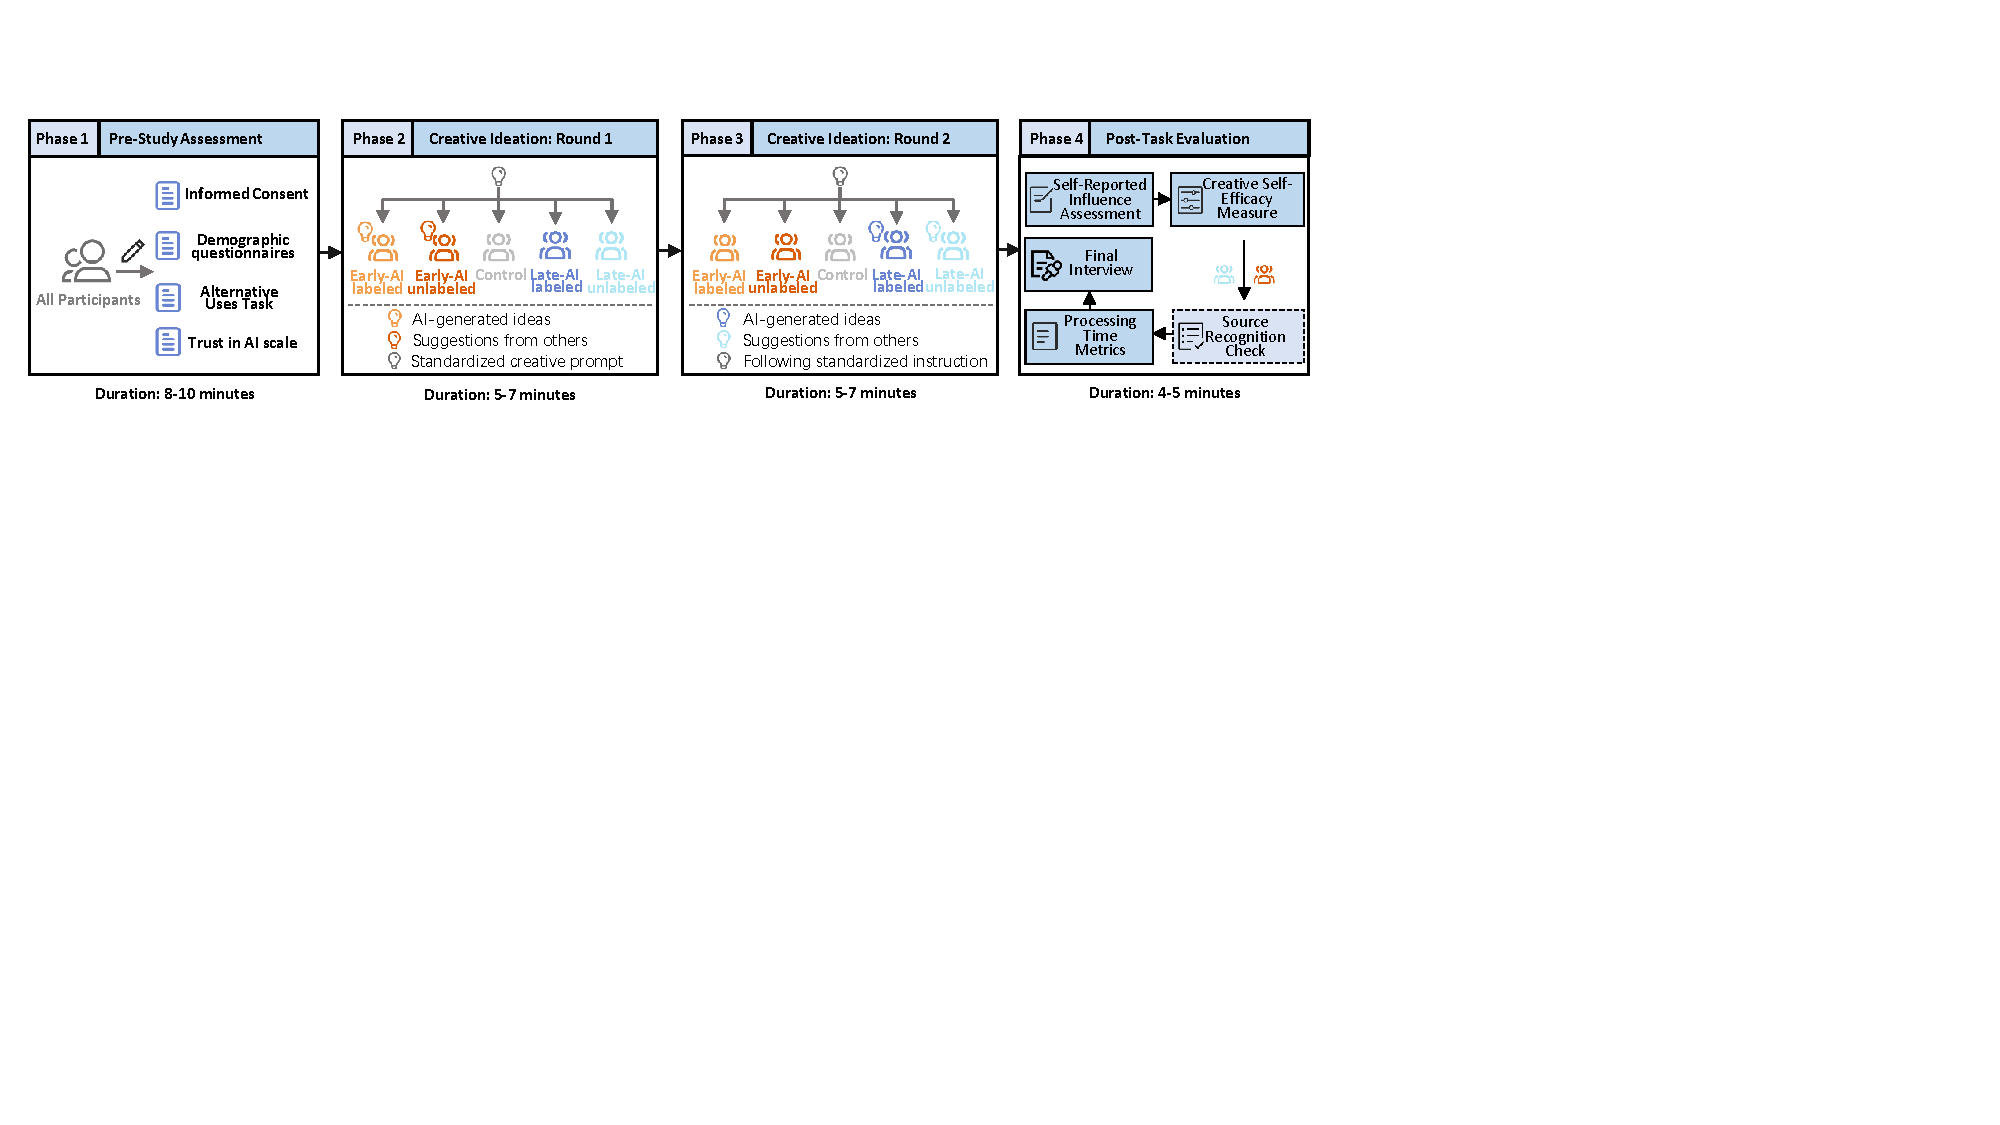
\includegraphics[width=1.0\textwidth]{method.pdf}}
\caption{Research procedure overview showing four phases: Pre-study Assessment (8-10 min), Creative Ideation Round 1 (5-7 min), Creative Ideation Round 2 (5-7 min), and Post-Task Evaluation (4-5 min). Each phase details key activities and participant group allocations for Early-AI, Late-AI, and Control conditions.}
\label{researchframework}
\end{figure*}
At the outset, participants completed a demographic form, followed by the Alternative Uses Task (AUT) to measure baseline creativity. They were asked to list as many unusual uses as possible for a “brick” within two minutes, and the total number of unique responses was used as an index of fluency. A Trust in AI scale, adapted from existing technology trust inventories~\cite{mcknight2011trust}, was also administered, although participants were not informed about the specific focus on AI until the debriefing phase.

In \textbf{Round 1}, all participants received the scenario prompt about reducing plastic pollution. Early-AI conditions were shown the GPT-4 suggestions here; Control and Late-AI conditions did not see any external suggestions during this stage. Participants had 5–7 minutes to type their solutions in an open text box that allowed them to refine their ideas before submission. 

In \textbf{Round 2}, participants were asked:

\textit{\textcolor{gray}{``Building upon your initial ideas, please refine, expand, or develop new solutions. Consider combining elements or exploring entirely new angles.”}}

Late-AI participants now received the same GPT-4 suggestions, again labeled or unlabeled according to condition. Early-AI and Control participants proceeded without new external inputs. After each round, a minimum response length of 50 words was enforced to ensure adequate engagement.

Following the ideation tasks, all participants completed a post-task evaluation that included: (a) a 7-point Likert item on perceived influence of external suggestions (for those who saw prompts), (b) a short creative self-efficacy scale adapted from~\cite{shaw2021measuring}, and (c) a brief source-recognition question for unlabeled groups to gauge whether they suspected an AI origin. A full debriefing explained the true source of the suggestions and the study’s purpose.

Twelve participants were then invited to a semi-structured interview (15–20 minutes) over videoconference. They represented low, moderate, and high baseline creativity scores, as well as a range of final idea originality. Interview prompts covered topics such as (1) “How, if at all, did the label ‘AI-generated’ or the lack of a label influence your willingness to accept or adapt these suggestions across multiple rounds?” and (2) “What factors led you to either follow the AI prompts more closely or diverge from them as you progressed to your final solution?” Interviewees were encouraged to elaborate on the details of their decision-making process, particularly any points at which they felt they “anchored” to AI-generated ideas or made a conscious “pivot.” They were also asked to reflect on whether labeling triggered shifts in trust, perceived legitimacy, or sense of authorship. All interviews were recorded, transcribed, and thematically analyzed. Figure \ref{researchframework} summarizes the conditions and procedure of this research.

\subsection{Measures}
Participants’ final submissions were rated using a modified Consensual Assessment Technique~\cite{baer2020consensual}. Three domain experts with backgrounds in environmental policy or innovation management independently assessed each final idea on novelty, usefulness, and originality, using 7-point scales. Inter-rater reliability was high (intraclass correlation $\ge$ 0.80) following a short calibration phase. To quantify participants’ alignment with GPT-4 suggestions, each submission was embedded via text-embedding-ada-002, and cosine similarities between the participant’s text and each AI suggestion were computed (lower distances indicated stronger overlap). Self-reported influence, creative self-efficacy, and source recognition data served as additional process measures.

\subsection{Data Analysis}
Initial data screening removed outliers (scores greater than three standard deviations from the mean) and incomplete responses. One-way and two-way analyses of variance tested main effects of timing and labeling on creativity ratings, semantic distances, and self-reported measures. Where indicated, Tukey’s HSD post-hoc tests were conducted, and effect sizes (partial $\eta^2$) were calculated. Mixed-effects models accounted for repeated measures within participants across the two rounds. Thematic analysis~\cite{braun2006using} was employed to examine the interview data, identifying patterns in participants’ attitudes about labeling, adoption of external prompts, and the perceived interplay between human and AI creativity.
\section{Results}
\begin{figure*}[htbp]
\centerline{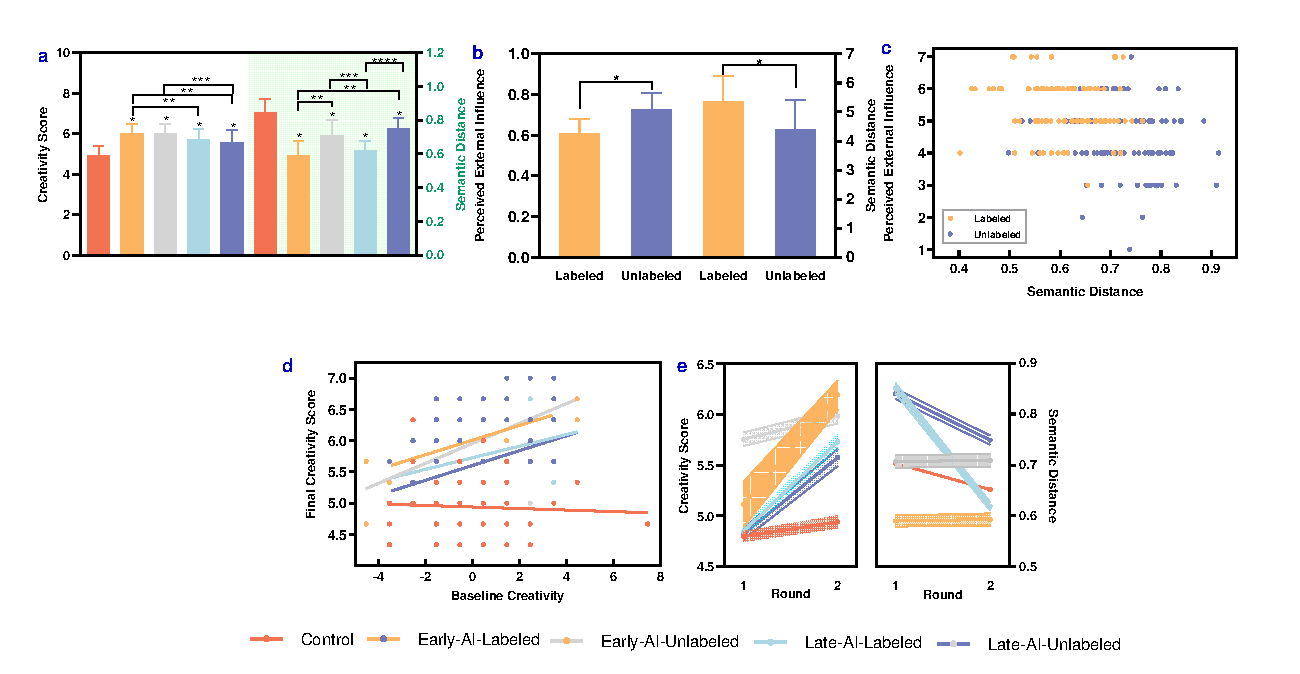
\includegraphics[width=1\textwidth]{resultfigure2.pdf}}
\caption{Results showing (a) creativity scores and semantic distances across conditions, (b) comparison of AI influence between labeled and unlabeled conditions, (c) correlation between semantic distance and perceived external influence, (d) interaction between baseline creativity and final creativity score, and (e) evolution of creativity scores and semantic distance across rounds. Shaded areas represent 95\% confidence intervals.}
\label{results1}
\end{figure*}

\subsection{RQ1 (Timing: Early vs. Late)} 
A one-way ANOVA examining final creativity scores (Figure~\ref{results1}a) indicated a significant main effect of condition, \(F(4, 237) = 37.54, p < .001\), partial \(\eta^2 = .38\). Post-hoc comparisons showed that both Early-AI groups surpassed the Late-AI groups and the Control in overall creativity, with Early-AI-Labeled achieving the highest mean (\(M = 6.01\), \(SD = 0.48\)) and the Control yielding the lowest (\(M = 4.94\)). A parallel ANOVA on semantic distance, \(F(4, 237) = 85.53, p < .001, \eta^2 = .59\), revealed that Early-AI-Labeled participants most closely aligned to the AI prompts (\(M = 0.59\)), whereas the Control remained the most divergent (\(M = 0.84\)). Additional component-wise analyses indicated robust differences for novelty \((F(4, 237)=30.75, p<.001)\) and usefulness \((F(4, 237)=51.64, p<.001)\), but not for originality \((F(4,237)=1.10, p=0.358)\). From an anchoring perspective, receiving AI early locked participants into those suggestions, boosting immediate creativity yet limiting autonomy. Late-AI groups, conversely, reported a more pronounced “pivot,” generating more divergent ideas than Early-AI but still exceeding the Control in final outcomes.

\subsection{RQ2 (Labeling: Labeled vs. Unlabeled)}
Compared to unlabeled prompts, labeled AI suggestions induced higher perceived external influence (PEI) (Figure~\ref{results1}b): \(M = 5.36\) vs. 4.39, \(t = 7.22, p < .001, d = 1.03\). Labeled participants also exhibited closer textual overlap with the AI (semantic distance of .61 vs. .73, \(t = -11.04, p < .001, d = 1.58\)). A negative correlation between PEI and semantic distance (Figure~\ref{results1}c), \(r = -0.35, p < .001\), implies that those who felt more influenced by the AI indeed integrated it more verbatim. Although labeling magnified reliance, 64\% of unlabeled participants correctly suspected the source was AI, suggesting that labeling is not solely responsible for recognition or adoption.

\subsection{RQ3 (Moderators: Baseline Creativity and Trust)}  
Moderation analyses indicated a significant interaction between baseline creativity and condition on final creativity, \(F(4, 237) = 4.42, p = .002\). As shown in Figure~\ref{results1}d and Table~\ref{tab:regression_slopes}, the slope of baseline creativity (AUT fluency) on final creativity was highest under Early-AI-Unlabeled (\(\beta = 0.159, SE = 0.033, p < .001\)) and Early-AI-Labeled (\(\beta = 0.117, SE = 0.035, p = .005\)), suggesting that participants with more initial flexibility capitalized on early AI prompts. In contrast, trust in AI did not exhibit a significant moderating effect (\(p > .17\)), implying that timing and labeling cues overshadowed general attitudes toward AI in a short-term creativity task.
\begin{table}
    \centering
    \begin{tabular}{llll}
        \hline
        Condition & Slope & SE & p-value \\
        \hline
        Control & -0.012 & 0.031 & 0.687 \\
        Early-AI-Labeled & 0.117 & 0.035 & 0.005 \\
        Early-AI-Unlabeled & 0.159 & 0.033 & $<.001$ \\
        Late-AI-Labeled & 0.093 & 0.037 & 0.029 \\
        Late-AI-Unlabeled & 0.118 & 0.036 & 0.005 \\
        \hline
    \end{tabular}
    \caption{Simple slopes indicating how baseline creativity relates to final creativity score in each condition}
    \label{tab:regression_slopes}
\end{table}

\subsection{RQ4 (Multi-round Evolution)} 
Comparisons of Rounds (Figure~\ref{results1}e) showed Late-AI participants demonstrating the largest boosts in creativity (increases up to \(+0.88\); \(t = -19.69, p < .001, d = 1.73\)) and the steepest declines in semantic distance (\(\Delta M = -0.23\)), consistent with a pronounced “pivot” once the AI prompts appeared. To assess these within-participant changes more rigorously, we used a repeated-measures ANOVA on creativity scores from Round 1 and Round 2, confirming that Late-AI conditions drove significantly larger improvements over time than their Early-AI or Control counterparts. Early-AI conditions achieved more modest progress from Round~1 to Round~2—e.g., Early-AI-Labeled improved by \(+0.17\)—reflecting the anchoring effect from seeing AI suggestions earlier. Meanwhile, the Control group changed minimally across rounds (\(+0.14\)), reinforcing that AI introduction (whether early or late) yields greater momentum than no AI at all. In practical terms, for instance, moving from an average creativity score of 4.94 (Control) to 6.01 (Early-AI-Labeled) suggests a substantial difference in idea quality as judged by experts, highlighting the applied significance of these numeric gains.

\subsection{Qualitative Interview Findings}
Thematic analysis of the semi-structured interviews revealed three main themes: (1) \emph{Awareness and Adaptation}, (2) \emph{Perceived Ownership and Authenticity}, and (3) \emph{Labeling-Triggered Reflection}. 

\paragraph{Awareness and Adaptation.} Several interviewees described an initial moment of \emph{“latching on”} to the AI idea when it appeared early, confirming the anchoring effect observed in our RQ1 results. One participant (P4) noted: \emph{“I felt I had a good starting point, so I built on the AI’s idea rather than reinventing the wheel.”}  Another participant (P11), who had professional experience in environmental advocacy, remarked, \emph{“I immediately recognized the AI’s approach as standard policy talk, so I tweaked it with on-the-ground examples.”} This adaptation echoes our finding that individuals with domain expertise are more inclined to integrate AI suggestions without feeling overshadowed. In contrast, individuals receiving suggestions late described a sense of \emph{“recalibration,”} wherein their initial self-driven ideas were suddenly enriched or redirected by the system. As one late-introduction participant (P9) put it, \emph{“I was already set on a certain path, but when I saw the AI suggestion, I realized there was an entirely different angle I could explore.” }These reflections align with our quantitative data showing that mid-process AI introduction can foster a pronounced pivot, offering novelty without fully overriding prior work.

\paragraph{Perceived Ownership and Authenticity.} While some participants perceived AI suggestions as creative catalysts, others expressed unease regarding authorship. P7 explained, \emph{“I’m proud of my final concept, but it’s hard to say how much was really me.”} This tension confirms the RQ3 insight that high-baseline-creativity users may seamlessly integrate external prompts without feeling overshadowed, whereas those less confident in their creative abilities experienced greater ambivalence. Another participant (P2) described actively \emph{“merging”} the AI’s idea with personal experiences, thus preserving a sense of \emph{“authentic authorship”} even when the AI had provided the core mechanism or structural concept. Such findings echo our moderation analyses, indicating that baseline creativity can buffer any perceived loss of originality.

\paragraph{Labeling-Triggered Reflection.} Consistent with RQ2, many participants remarked that explicit AI-generated labeling led them to scrutinize the suggestions more carefully, weighing factors like novelty or \emph{“robotic tone.”} P12 recounted, \emph{“Seeing the label made me both more curious and more critical. I wanted to double-check if it was just generic filler.”}  Others in unlabeled conditions (e.g., P8) reported a \emph{“strong hunch”} that the suggestions were AI-generated, but felt uncertain whether acknowledging it would bias them. This illustrates how labeling can heighten meta-cognitive assessments of the prompt’s credibility, especially when participants suspect an algorithmic source. Intriguingly, even unlabeled participants reported noticing phrases that felt \emph{“computational,”} which prompted some to guess the source. This observation supports the survey result that 64\% of unlabeled recipients suspected an AI origin. Nevertheless, labeling also heightened users’ sense of external guidance, confirming our correlation finding (PEI vs. semantic distance) that greater reported reliance translates to closer textual overlap. Ultimately, these interviews demonstrate that labeling not only boosts awareness but spurs deeper reflection and adaptive strategizing—participants either anchored more decisively if they deemed the AI idea credible or pivoted away if the AI content felt misaligned with their personal objectives.

\section{Discussion}

Our findings illustrate that \textit{when} and \textit{how} AI suggestions are introduced can substantially alter multi-round creative ideation, a result that resonates with prior claims about iterative thinking~\cite{tolkamp2023creativity,zamani2022closer} and the broader potential of generative AI in supporting human creativity~\cite{epstein2023art,kwon2024designer,reeves2024generative}. By showing that early prompts lead to stronger anchoring effects yet also raise immediate creativity, whereas late prompts trigger a salient mid-process pivot, this study contributes a more nuanced view of how human–AI synergy unfolds. From a human-centred AI perspective, these insights underscore the importance of designing generative systems that mindfully time their suggestions—an approach that can encourage either rapid convergence (early introduction) or strategic redirection (late introduction), depending on users’ needs and context.

The anchoring vs. pivot phenomenon—grounded in both cognitive anchoring theory~\cite{tversky1974judgment} and dual-process frameworks~\cite{kahneman2011thinking}—illuminates key pathways by which AI can influence, guide, or constrain creative thought. Early introduction often “locks in” the user to the first set of ideas, fostering synergy but potentially narrowing subsequent exploration. Conversely, late prompts appear to spark a more robust reorientation, echoing research in organizational creativity indicating that fresh external input can catalyze radical shifts~\cite{harvey2014creative}. This anchoring/pivot dynamic suggests that designers of AI ideation tools could intentionally display suggestions at selective intervals—such as mid-way through a brainstorming session—to balance initial self-driven exploration with a carefully timed injection of novel perspectives.

In tandem with the timing results, our labeling manipulation reveals how explicit attribution of AI origin elevates perceived external influence and fosters deeper semantic overlap. On one hand, labeling can foster transparency and user awareness, aligning with calls for ethical AI design in high-stakes contexts~\cite{bankins2024multilevel,dietvorst2015algorithm}. On the other, unlabeled suggestions offer a frictionless experience that some might prefer for rapid brainstorming but raises questions about authorship, intellectual property, and the user’s “right to know” the source of ideas. Our study further shows that many participants can detect AI output even without labels, suggesting that transparency alone might not fully resolve issues of algorithmic accountability. A tension thus arises between frictionless usage and ethical disclosure—a dilemma echoed in discussions of responsible AI usage, particularly when users’ creative autonomy is at stake.

Although our experimental task focused on reducing plastic pollution in urban environments, these findings likely generalize to a spectrum of creative or problem-solving domains that hinge on iterative refinement—product design, educational technology, policy brainstorming, and more. Moreover, the observed “creative pivot” effect could feasibly extend to multi-session or multi-day processes. Future research might explore whether repeated pivot opportunities—offered by staggered AI prompts across multiple sessions—further amplify creativity or risk saturating users with external suggestions. As modern workplaces increasingly adopt AI-based co-creative tools~\cite{ma2024human,fui2023generative}, timed prompts and explicit labeling become critical design levers for harnessing AI’s breadth of knowledge while preserving user autonomy. Educational applications could, for instance, insert AI “nudges” midway through student projects to spur novel directions rather than overshadow their initial, self-driven exploration. In organizational innovation contexts, managers or team leaders might deploy late-phase AI interventions to combat creative inertia, effectively reinvigorating group ideation processes. The capacity for multi-round synergy—rather than a single-shot query-and-response—may prove essential for addressing real-world problems of greater complexity and uncertainty.

Several avenues invite further exploration. First, this study constrained ideation to two rounds of brainstorming. In real-world settings, creative processes can extend over multiple days or weeks, potentially yielding deeper “momentum transfer” or even saturation effects after repeated AI interactions. Future work could thus investigate how subsequent cycles of human–AI interplay transform user acceptance, trust, and sense of creative ownership over longer timelines. Second, domain-specific tasks—for instance, engineering design or policy drafting—would refine our understanding of how subject-matter expertise intersects with AI reliance: highly skilled users may harness AI suggestions more selectively, whereas novices might rely on them wholesale. Third, longitudinal studies could address how repeated exposure to AI suggestions recalibrates user trust, especially if the AI’s performance varies or if transparency cues shift. This richer understanding would inform guidelines for responsibly implementing multi-stage AI support in a range of professional and educational contexts.

Our design relied on a relatively short time frame (two 5–7-minute rounds), a convenience sample, and a single creative domain. While these conditions afforded experimental control, they temper the immediate extension of our results to longer, more complex creative endeavors. Moreover, factors like risk perception or cultural attitudes toward technology could modulate labeling effects. Nonetheless, the consistency of our anchoring vs. pivot findings, coupled with clear labeling impacts, underscores the robustness of the core phenomena. By integrating real-time user feedback mechanisms—like dynamic trust or engagement metrics—future systems could tailor the timing and transparency of AI suggestions to maximize synergy without eroding human autonomy.

Our findings offer several takeaways for broader co-creative AI research and real-world application. First, they emphasize the timing of AI suggestions as a key design lever: while early prompts can scaffold novices or users with lower baseline creativity, more advanced users may benefit from staggered prompting to preserve initial autonomy and spark mid-process pivots. Second, the labeling of AI output has direct relevance to ongoing policy debates about transparency and accountability (e.g., within the EU AI Act). Encouraging explicit disclosure can increase perceived influence and user scrutiny, yet many participants still suspected AI origins even without overt labeling. Finally, practitioners developing AI-assisted creativity tools might adopt an adaptive approach that tailors prompt timing and labeling cues to user characteristics. By embedding real-time feedback or self-assessment modules, systems could identify moments of creative impasse and strategically deploy a “late AI nudge,” thereby balancing efficiency gains with the user’s sense of ownership. Such tactics extend beyond plastic pollution to any domain—such as product design or educational scaffolding—where iterative ideation and user-driven exploration remain paramount.

\section{Conclusion}
This work sheds new light on the ways in which AI-generated prompts can shape iterative creativity over multiple rounds of ideation. By systematically examining the roles of timing (early vs. late introduction) and labeling (AI-labeled vs. unlabeled) in a controlled experiment, we highlight how AI can both anchor human thinking from the start and pivot it toward novel directions at later stages. Early introduction was shown to boost creativity levels rapidly, albeit at the cost of stronger anchoring, while late introduction triggered more radical shifts and improvements in subsequent rounds. Labeling effects further underscored how explicit attribution intensified perceived influence and textual overlap, yet left important ethical questions regarding authorship, transparency, and user autonomy.

These insights have direct implications for the design of next-generation AI creativity tools. In particular, they suggest that developers should consider adaptive strategies that incorporate user-driven exploration, mid-process AI “nudges,” and transparent labeling mechanisms that balance efficiency with ethical responsibilities. Moreover, the interviews revealed that users’ baseline creativity partly governs their receptiveness to AI suggestions, extending our understanding of how individual differences intersect with algorithmic input. By capturing both anchoring and pivot effects within multi-round ideation, this study not only refines theoretical models of human–AI synergy but also points to practical guidelines for implementing AI support in diverse, creativity-intensive domains such as design, innovation management, and educational technology.

%% The file named.bst is a bibliography style file for BibTeX 0.99c
\bibliographystyle{named}
\bibliography{ijcai25}

\end{document}

 